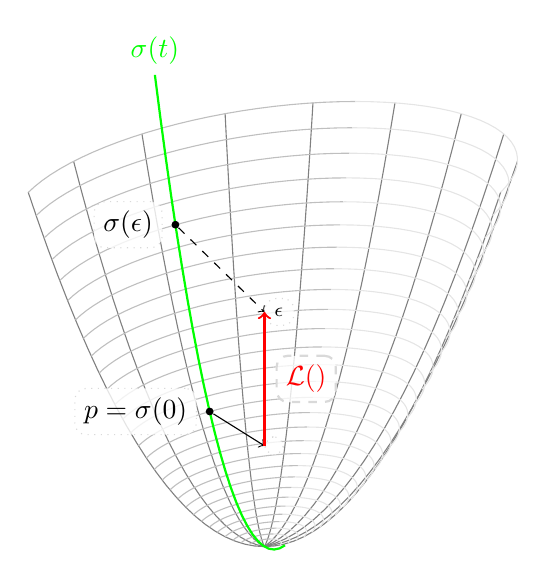
\begin{tikzpicture}[declare function={f(\n)=\n*\n;}, scale=2, 
	back/.style={ rounded corners, fill opacity=0.8, text opacity=1, fill=white, dotted, draw=gray!30!white}]

\foreach \a in {90, 110, ..., 270}
	\draw[gray, variable=\x, domain=0:1.5] plot ({\x * sin(\a)}, {f(\x)}, {\x * cos(\a)});

\foreach \r in {0.1,0.15,...,1.5}
{
	\draw[gray!50!white, variable=\x, domain=pi:3*pi/2] plot ({\r * sin(\x r)}, {f(\r)}, {\r * cos(\x r)});
	\draw[gray!20!white, variable=\x, domain=pi/2:pi] plot ({\r * sin(\x r)}, {f(\r)}, {\r * cos(\x r)});
} 

\pgfmathsetmacro{\r}{0.8}	
\pgfmathsetmacro{\a}{225}
\pgfmathsetmacro{\x}{\r * sin(\a)}
\pgfmathsetmacro{\y}{\r * cos(\a)}
\pgfmathsetmacro{\z}{f(\r)}

\draw[green, thick, variable=\x, domain=-0.3:1.6] plot ({\x * sin(\a)}, {f(\x)}, {\x * cos(\a)}) node[above] {$\sigma(t)$};

\node[circle, fill, black, inner sep=1pt, label={[back, xshift=-3]left:$p=\sigma(0)$}] (P) at (\x, \z, \y) {};
\coordinate (N) at (0, {f(\r)}, 0);
\draw[->] (P) -- (N)  node[right, back] {$\vn$};

\pgfmathsetmacro{\r}{1.3}
\pgfmathsetmacro{\x}{\r * sin(\a)}
\pgfmathsetmacro{\y}{\r * cos(\a)}
\pgfmathsetmacro{\z}{f(\r)}

\node[circle, fill, black, inner sep=1pt, label={[back, xshift=-3]left:$\sigma(\epsilon)$}] (PN) at (\x, \z, \y) {};
\coordinate (NN) at (0, {f(\r) - 0.2}, 0);
\draw[dashed, ->] (PN) -- (NN) node[right, back] {$\vn_\epsilon$};

\draw[thick, red,->] (N) -- node[midway, right, back, dashed, xshift=4] {$\mathcal{L}(\vv)$} (NN);

\end{tikzpicture}